\chapter{System Design}
\label{chap:design}
\setlength{\parskip}{1em}

\section{Technology Stack Selection}

Technology selection was governed by four criteria: team competency,
documentation quality, open-source licence compatibility, and architectural
fit with the monolithic pattern. The \Cref{tab:techstack} presents the selected
stack with rationale.

\begin{table}[H]
  \centering
  \caption{TinyCRM technology stack}
  \label{tab:techstack}
%  \setstretch{1.1}
  \begin{tabularx}{\textwidth}{@{}L{2.6cm} L{2.4cm} C{1.3cm} X@{}}
    \toprule
    \thead{Layer} & \thead{Technology} & \thead{Version} &
    \thead{Rationale} \\
    \midrule
    Backend framework & FastAPI & 0.136.1 &
      ASGI-native, async support, automatic OpenAPI schema generation,
      high performance \\
    ORM & SQLAlchemy & 2.0.49 &
      Mature, expressive, supports async sessions via \texttt{asyncpg} \\
    ML library & scikit-learn + XGBoost + SHAP & 1.8.0 / 3.2.0 / 0.51 &
      Mature pipelines, SHAP for explainability \\
    Frontend & Vue.js~3 & 3.5.33 &
      Composition API, progressive framework, large ecosystem \\
    UI components & Vuetify~3 & 3.5 &
      Material Design, comprehensive data-table and chart support \\
    State management & Pinia & 2.1 &
      Lightweight, TypeScript-friendly successor to Vuex \\
    Database & PostgreSQL & 18 &
      ACID compliance, JSONB support, QazCloud managed service \\
    Background tasks & FastAPI \texttt{BackgroundTasks} & built-in &
      In-process async task dispatch for batch ML inference and deferred
      email; avoids additional broker infrastructure \\
    Containerisation & Docker + Compose & 29.4.2 / 2.40 &
      Reproducible deployments, QazCloud container support \\
    Web server & Nginx + Uvicorn & 1.30 / 0.46 &
      Production-grade ASGI serving \\
    CI/CD & GitHub Actions & -- &
      Free tier, YAML pipeline, Docker Hub integration \\
    API documentation & FastAPI built-in (OpenAPI 3.0) & -- &
      Automatic schema from type annotations \\
    \bottomrule
  \end{tabularx}
\end{table}

\subsection{Backend Framework Comparison}

Three Python web frameworks were evaluated for the backend role:
FastAPI, Django with Django REST Framework (DRF), and Flask. The
comparison is presented in \cref{tab:frameworkcomp}.

\begin{table}[H]
  \centering
  \caption{Backend framework comparison}
  \label{tab:frameworkcomp}
%  \setstretch{1.1}
  \begin{tabularx}{\textwidth}{@{}L{3.0cm} L{2.8cm} L{2.8cm} L{2.8cm}@{}}
    \toprule
    \thead{Criterion} & \thead{FastAPI} & \thead{Django + DRF} &
    \thead{Flask} \\
    \midrule
    Native async support & Full (ASGI) & Full (ASGI) & Limited (WSGI) \\
    Auto OpenAPI schema & Built-in & Via drf-spectacular & Via flasgger \\
    Built-in ORM & No (SQLAlchemy) & Django ORM & No (SQLAlchemy) \\
    Type-safety & Strong (Pydantic) & Serialisers & Manual \\
    Performance & Very high & Moderate & High \\
    Built-in admin & No & Yes & No \\
    Team familiarity & High & Medium & Low \\
    Verdict & \textbf{Selected} & Runner-up & Not selected \\
    \bottomrule
  \end{tabularx}
\end{table}

FastAPI was selected for its native ASGI async support (beneficial for
concurrent ML inference requests), automatic OpenAPI~3.0 schema generation
from Python type annotations, and Pydantic-based request/response
validation. SQLAlchemy~2.0's async session interface
(\texttt{AsyncSession} with \texttt{asyncpg}) complements FastAPI's async
model and provides an expressive, database-agnostic ORM layer. The absence
of a built-in admin interface, a notable advantage of Django, is mitigated
by the use of pgAdmin and direct API access during development.

\section{High-Level Architecture}

TinyCRM follows a three-tier monolithic architecture: a presentation
tier (Vue.js~3 SPA), an application tier (FastAPI monolith with embedded
Celery worker), and a data tier (PostgreSQL~15 with Redis~7 cache).
The ML pipeline is embedded within the FastAPI application as a dedicated
router module, with trained models serialised to disk using \texttt{joblib}
and loaded into memory at application start-up. The rationale for embedding
rather than externalising the ML models is consistent with the
``monolith first'' principle \citep{fowler2014microservices}: the extraction
boundary is clearly defined (the \texttt{/ml} router) and can be promoted
to an independent microservice in a future iteration.

\begin{figure}[H]
{
\centering
\begin{subfigure}{1 \textwidth}
    \centering
    {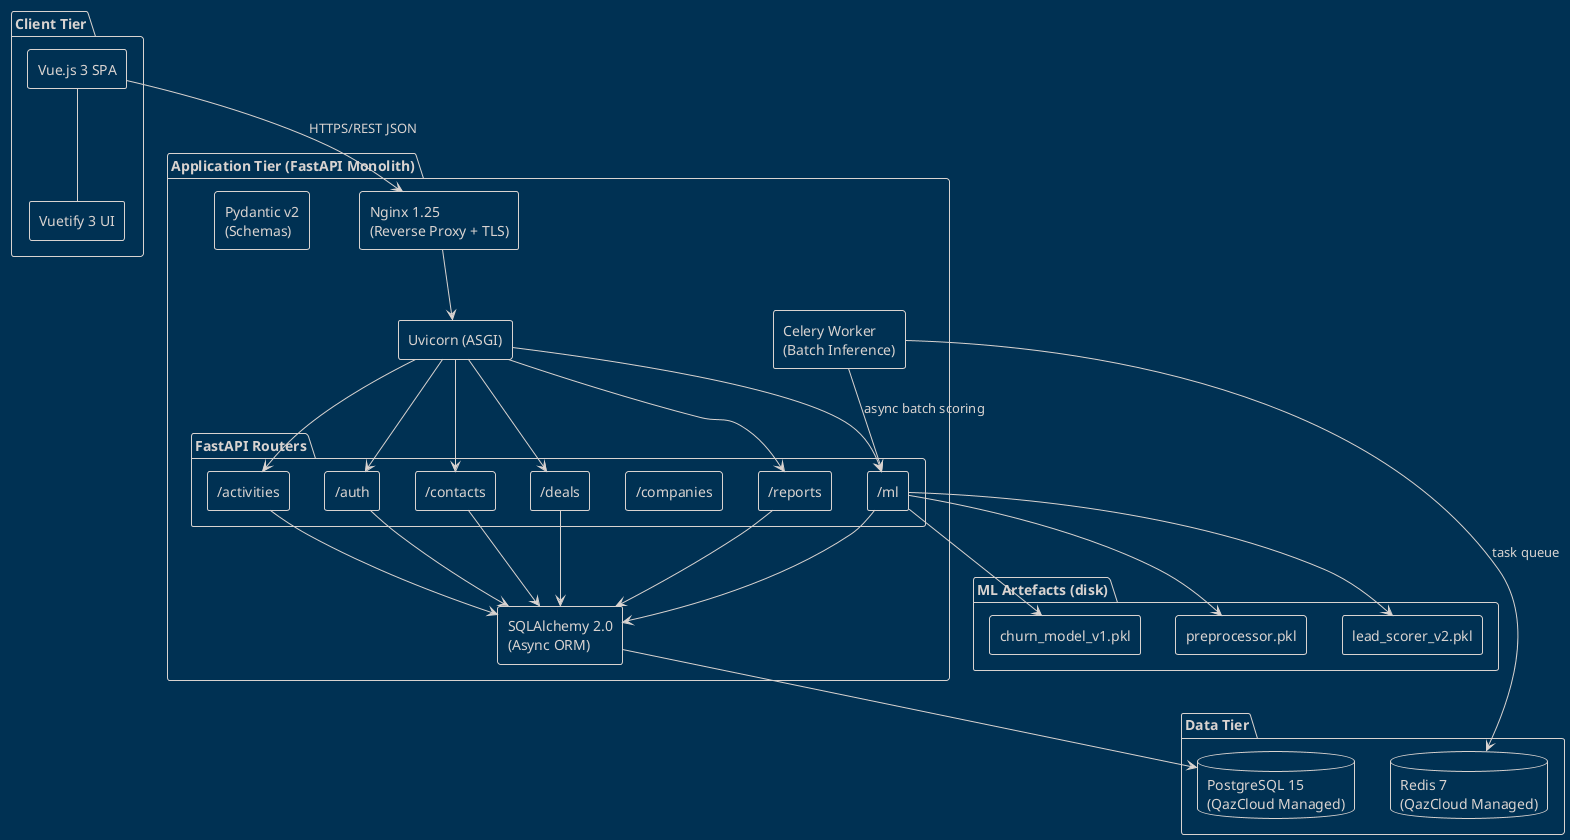
\includegraphics[width=\textwidth]{chapters/chapter04/fig/component_diagram.png}
    \caption{}\label{Fig.4.1.a}}
\end{subfigure}
%
\caption{Component diagram of the project.}
\label{Fig.4.1}
}
\end{figure}
